\documentclass[a4paper, 10pt]{article}
\usepackage{enumitem}
\usepackage{tikz}
\usepackage{lmodern}


\begin{document}
\textsc{\bfseries\huge Exercice 18}
\begin{enumerate}
	\item Pour lier (a,b) à (c,d), c-a+d-b étapes sont toujours nécéssaires. \\ \\
	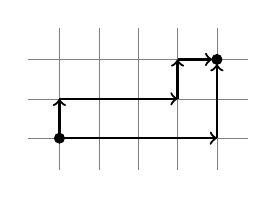
\begin{tikzpicture}
		\draw[step=0.5cm,gray,very thin] (-1.9,-0.9) grid (0.9,0.9);
		\fill (-1.5,-0.5) circle[radius=2pt];
		\fill (0.5,0.5) circle[radius=2pt];
		\draw[thick,->] (-1.5,-0.5) -- (0.5,-0.5);
		\draw[thick,->] (0.5,-0.5) -- (0.5,0.44);
		\draw[thick,->] (-1.5,-0.5) -- (-1.5,0);
		\draw[thick,->]  (-1.5,0) -- (0,0);
		\draw[thick,->] (0,0) -- (0,0.5);
		\draw[thick,->] (0,0.5) -- (0.44,0.5);
	\end{tikzpicture} 
	
	\item Notons M l'instruction <<monter>> et D l'instruction <<aller a droite>>. 
	Soit n un entier naturel. Un chemin valide joignant (0,0) à (n,n) est un <<mot>> de longeur \(n-0+n-0 = 2n\) comportant n fois la lettre M (Voir l'exercice 11).
	Il y a donc \(2n\choose n\) chemins.
	
	\item La condition \(a \leq b\) pour tout somment (a,b) équivaut à ce que les chemins soient restreints à la partie du graphe située au dessus de la diagonale ((0,0),(n,n))
	À partir de petits schémas, on determine à la main que \(c_{0} = 1,c_{1} = 1, c_{2} = 2, c_{3} = 5\) et \( c_{4} = 7\) 
	
		\foreach \n in {0.5,1,...,2}{
			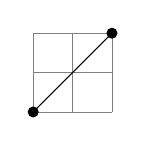
\begin{tikzpicture}
			\draw[step=0.5cm,gray,very thin] (0,0) grid (\n,\n);
			\fill (0,0) circle[radius=2pt];
			\fill (\n,\n) circle[radius=2pt];
			\draw (0,0) -- (\n,\n);
			\end{tikzpicture}}  À remplir !
	
	\item Soit n un entier naturel. Trions les chemins joignant (0,0) et (n,n) en fonction des points en contact avec la diagonale :
	\begin{enumerate}
		\item Si un chemin n'est en contact qu'avec les points (0,0) et (n,n), alors il y à \(c_{n-1}\) possibilitées.
		\item Sinon, on trie les chemins en fonction du premier point de contact. Si le premier point de contact est (m,m),
		il y a \(c_{m-1}\) possibilitées car il faut poser un nouvelle diagonalle  pour ne pas croiser l'ancienne. 
			Il y a ensuite \(c_{n-m}\) chemins possible, qui peuvent passer par la diagonale, pour clore le trajet. 
	\end{enumerate}
	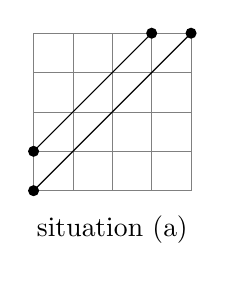
\begin{tikzpicture}
		\draw[step=0.5cm,gray,very thin] (0,0) grid (2,2);
		\fill (0,0) circle[radius=2pt];
		\fill (2,2) circle[radius=2pt];
		\draw (0,0) -- (2,2);
		\fill (0,0.5) circle[radius=2pt];
		\fill (1.5,2) circle[radius=2pt];
		\draw (0,0.5) -- (1.5,2);
		\node[draw=none] at (1,-0.5) {situation (a)};
	\end{tikzpicture}
	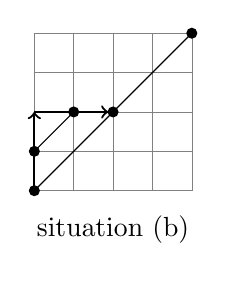
\begin{tikzpicture}
		\draw[step=0.5cm,gray,very thin] (0,0) grid (2,2);
		\fill (0,0) circle[radius=2pt];
		\fill (2,2) circle[radius=2pt];
		\draw (0,0) -- (2,2);
		\fill (1,1) circle[radius=2pt];
		\fill (0.5,1) circle[radius=2pt];
		\fill (0,0.5) circle[radius=2pt];
		\draw (0,0.5) -- (0.5,1);
		\draw[thick,->] (0,0) -- (0,1);
		\draw[thick,->] (0,1) -- (0.94,1);
		\node[draw=none] at (1,-0.5) {situation (b)};
	\end{tikzpicture}
		
		Finalement, on obtient \(\(c_{n} = c_{n-1} +\sum_{1}^{n} c_{m-1} \times c_{n-m} = \sum_{0}^{n} c_{m-1} \times c_{n-m} \). 
	
	\item Soit n un entier naturel. \(2n\choose n\) est le nombre total de chemin joignant (0,0) et (n,n). Or, il existe au moins un chemin valide passant sous la diagonale (le mot formé de n D puis de n M).
	On a donc nécessairement \(c_{n} \leq \) \(2n\choose n\).

	%%%%%%%%%%%%%%%%%%%%%%%%%%%%%%% Deuxième partie %%%%%%%%%%%%%%%%%%%%%%%%%%%%%%%%%%%%%

	\item Soit n un entier naturel. \(c_{n} \) est égal à la somme de tous les chemins valides minus ceux qui passent sous la diagonale. 
	Intéressons nous à ces dernier et notons \( b_{n} \) leur nombre. Un tel chemin coupe nécessairement la droite y = x - 1.
	Soit k un entier naturel inferieur à n. Lorsque un chemin coupe cette droite au point (k+1,k), il faut encore monter n-k fois et avancer n-k-1 fois pour atteindre le point (n+1,n+1). Si on inverse à partir du \(2 \times k +1\)-ième caractère les lettres M et D dans le mot associé au chemin, on obtient un nouveau chemin joignant (0,0) et (k+1 + n-k,k + n-k-1)=(n+1,n-1)).\\

\begin{minipage}[c]{3.5cm}	
	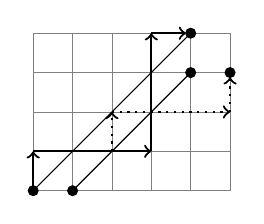
\begin{tikzpicture}
		\draw[step=0.5cm,gray,very thin] (0,0) grid (2.5,2);
		\fill (0,0) circle[radius=2pt];
		\fill (2,2) circle[radius=2pt];
		\draw (0,0) -- (2,2);
		\fill (0.5,0) circle[radius=2pt];
		\fill (2,1.5) circle[radius=2pt];
		\draw (0.5,0) -- (2,1.5);
		\draw[thick,->] (0,0) -- (0,0.5);
		\draw[thick,->] (0,0.5) -- (1.5,0.5);
		\draw[thick,->] (1.5,0.5) -- (1.5,2);
		\draw[thick,->] (1.5,2) -- (1.94,2);
		
		\fill (2.5,1.5) circle[radius=2pt];
		\draw[thick,dotted,->] (1,0.5) -- (1,1);
		\draw[thick,dotted,->] (1,1) -- (2.5,1);
		\draw[thick,dotted,->] (2.5,1) -- (2.5,1.44);
	\end{tikzpicture}
\end{minipage}	
\begin{minipage}[c]{7cm}
	\(MDD-DMMMD \mapsto  MDD-MDDDM\)\\
	\(MDD-MDDDM \mapsto  MDD-DMMMD\)
\end{minipage}\\
 
	Notons \(\delta_{k}\) l'application effectant cette opération à partir du k-ieme caractère, \(\phi_{1}\) la bijection associant à un chemin son mot et \(\psi\) l'application associant à un mot le plus petit entier k tel qu'il y ait dans les k-1 premieres lettres du mot une lettre D supplémentaire par rapport au nombre de lettre M. \(\Omega := \delta_{\psi \circ \phi_{1}} \circ \phi_{1}\) est bien défine et involutive (et donc une bijective), de \(E_{1}\) := l'ensemble des chemins coupant la droite y = x - 1 vers \(E_{2\)l'ensemble des chemins joignant (0,0) et (n+1,n-1):
	\begin{itemize}
		\item[--] \(\delta_{k}\) est une involution pour tout entier naturel k inferieur à n.
		\item[--] \(\psi\) est bien définie puisque les chemins coupent y = x-1 (par hypothèse pour le sens direct et car ils joignent (0,0) et (n+1,n-1) pour la réciproque), et pour tout mot M, \(\psi(M) = \psi(\Omega(M)) \) car la premiière partie du mot est justement laissée inchangée.
		\item[--] \(\Omega\) est alors bijective car tout élément de \(E_{2}\) admet un antécedant : Son image par \(\Omega\), et injective, par unicité de l'image par \(Omega\) d'un élement de E2.
	
	\end{itemize}

	Finalement, \(b_{n}\) étant le nombre de chemins joignants (0,0) et (n+1,n-1) (égal au nombre de mots à 2n lettres comprenants n-1 lettres M), on obtient bien 
	\( c_{n} = \)\( 2n\choose n\)\(+ b_{n} = \)\( 2n\choose n\)+\( 2n\choose n-1\)

	\item Notons \(p_{n}\) le nombre de façon de <<bien parenthèser>> un expression avec n paire de parenthèses.
	Pour montrer que \(p_{n} = c_{n}\), on pourrait montrer que \(p_{0} = c_{0}\) et que l'on a la même relation de récurence avec les \(p_{0}\), mais il suffit de construire une bijection entre les chemin joignant (0,0) et (n,n) en passant au dessus de la diagonale et les parenthèsages d'expression avec n paire de parenthèses. \\ 
	On peut representer un parenthèsage comme un mot de longueur 2n comportant n fois la lettre <<(>> et n fois la lettre <<)>>, et pour que le parenthèsage soit correct, en parcourant le mot de gauche à droite il ne doit pas y avoir strictement plus de <<)>> que de <<(>>. Or les chemins étudiée sont aussi représentés par des mots (question 2.). La condition \(a \leq b \) pour tout sommet (a,b) impose de plus de l'on compte plus de lettre M que de lettre D en parcourant de gauche à droite les mots représentant les chemins.
	\\ \\ Notant \(\phi_{2}\) la bijection associant à un parenthèsage son mot et \(\Delta\) la bijection échangant les lettres M et <<(>> et les lettres D et <<)>>, la bijection recherché est alors :
	\( \phi_{1}^{-1} \circ \Delta \circ \phi_{2}\)}


\end{enumerate}
\end{document}
